\section{Validation}
We use the following constants:
\begin{align}
d_\text{max}^\text{transition} &= \SI{1}{\milli\meter} \\
d^\text{discretization} &= \SI{0.2}{\milli\meter} \\
t_\text{beading} &= \SI{0.4}{\milli\meter} \\
d_\text{max}^\text{intersection} &= \SI{75}{\percent}
\end{align}

We use a transition anchor position of
%$$t_-(n) =  t(n) \frac{ b^{-1}(n) - p(n) }{p(n+1) - p(n) }$$
%$$t_-(n) =  t(n) \frac{ b^{-1}(n) - 0.4n }{0.4(n+1) - 0.4n }$$
%$$t_-(n) =  t(n) \frac{ b^{-1}(n) - 0.4n }{0.4}$$
$$t_0(n) =  t(n) \left( b^{-1}(n) / 0.4  - n \right)$$
This should ensure that the transitions never overlap with the locations $v$ where $2 R(v) = 0.4n$ for $n \in \mathbb{N}$, since \SI{0.4}{\milli\meter} is the prefered bead width for a similar nozzle size.

Our beading strategies are based on a prefered width $w_\text{pref} = \SI{0.4}{\milli\meter}$, which is equal to the size of the hole in the printing nozzle.

We set 
\begin{align*}
t(n) &= w_\text{pref} \\
\alpha_\text{max} &= \SI{135}{\degree} \\
L(n,d)_i &= 
\begin{cases}
-\frac12 W(n,d)_i + \sum_{j=0}^i W(n,d)_j & \text{ if } i < \frac12 (n -1) \\
d/2 & \text{ if } i =  \frac12 (n -1) \\
d - W(n,d)_{n-1-i} & \text{ otherwise }\\
\end{cases}
\end{align*}


\begin{figure*}
\centering
\setlength{\figwidth}{0.19\textwidth}
\setlength{\figheight}{0.283\textwidth}
\begin{subfigure}{\figwidth}\centering
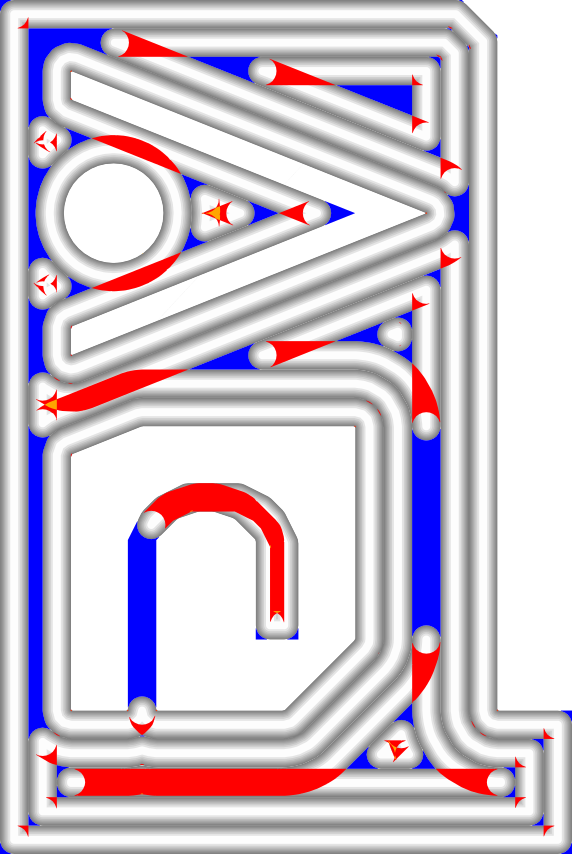
\includegraphics[height=\figheight]{sources/validation/gMAT_example/TEST_naive_accuracy.png}
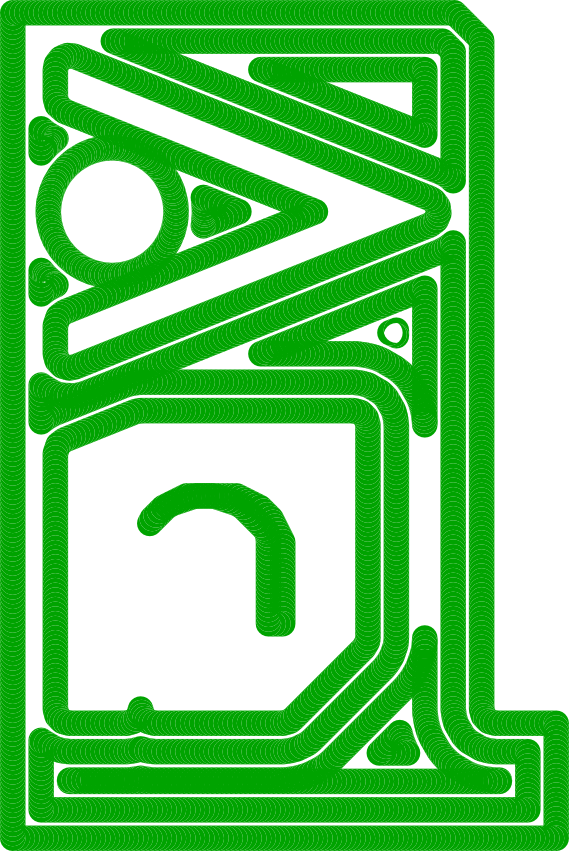
\includegraphics[height=\figheight]{sources/validation/gMAT_example/TEST_naive_widths.png}
\caption{Naive}\label{TEST_naive_accuracy}
\end{subfigure}
%\begin{subfigure}{\figwidth}\centering
%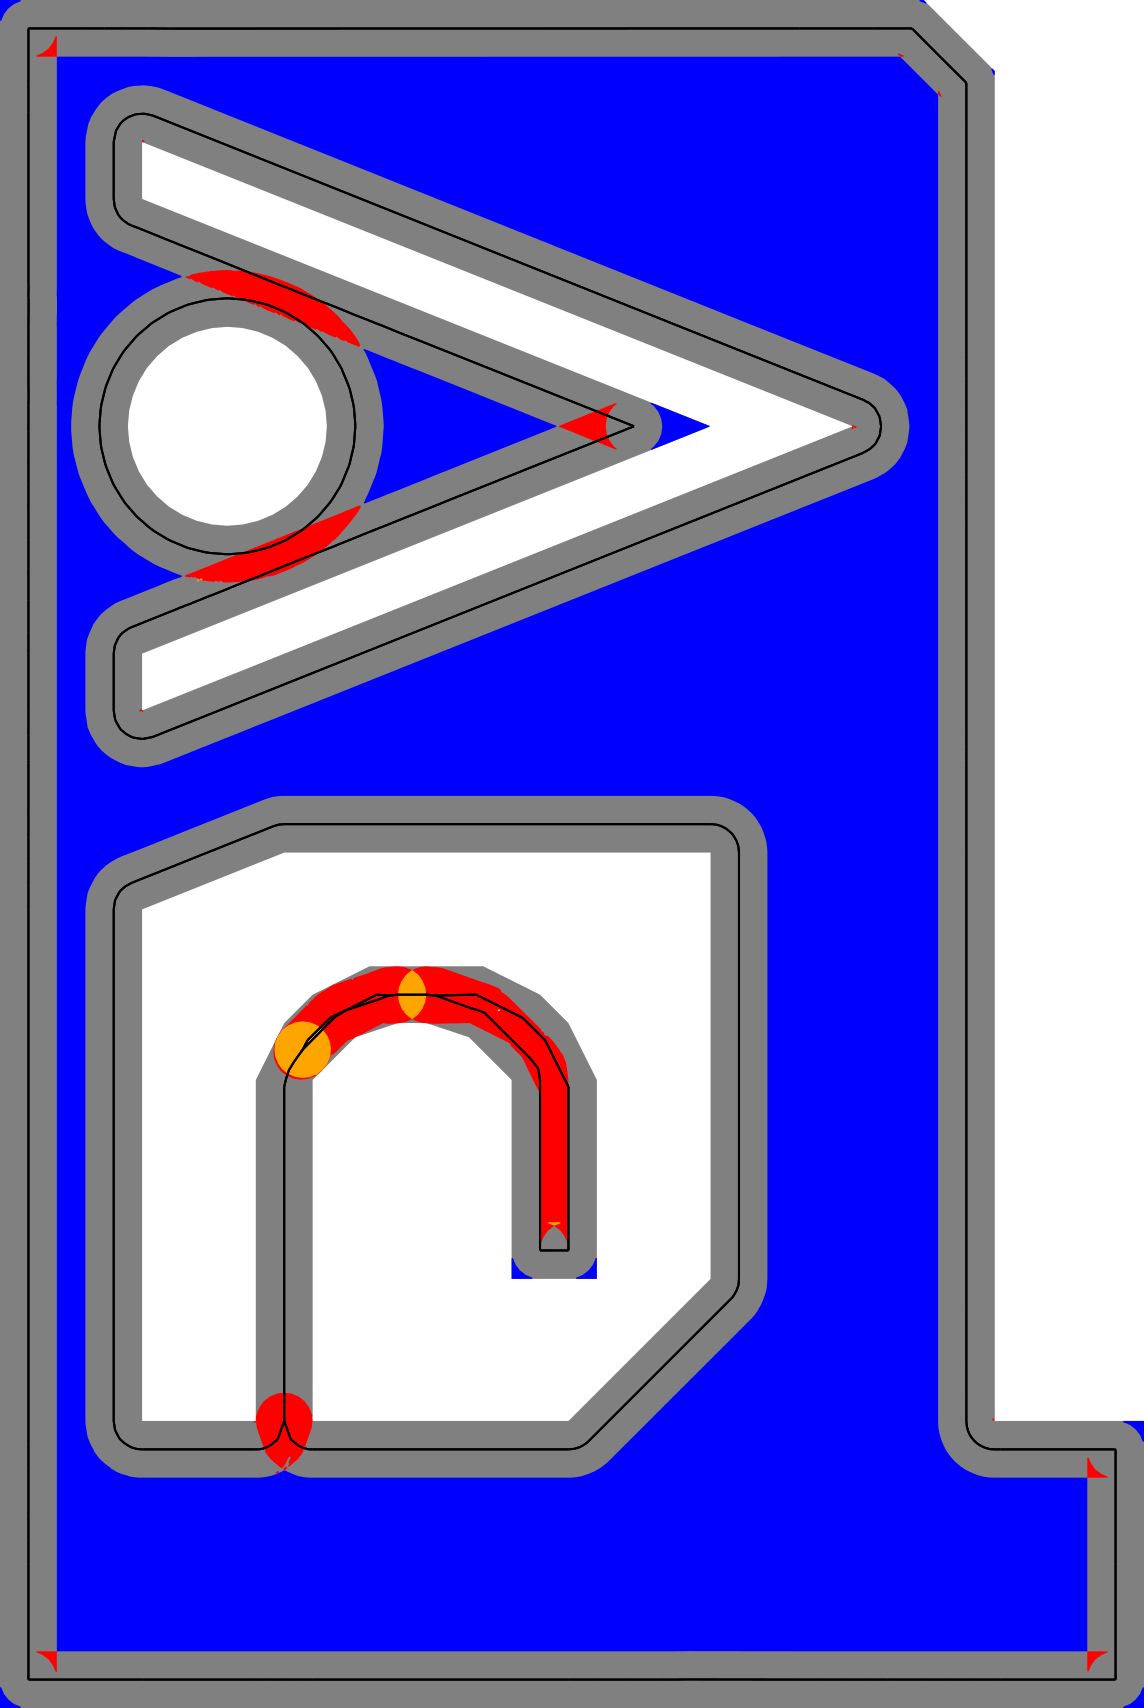
\includegraphics[height=\figheight]{sources/validation/gMAT_example/TEST_SingleBead_accuracy.png}
%
\includegraphics[height=\figheight]{sources/validation/gMAT_example/TEST_SingleBead_widths.png}
%\caption{Single}\label{TEST_SingleBead_accuracy}
%\end{subfigure}
\begin{subfigure}{\figwidth}\centering
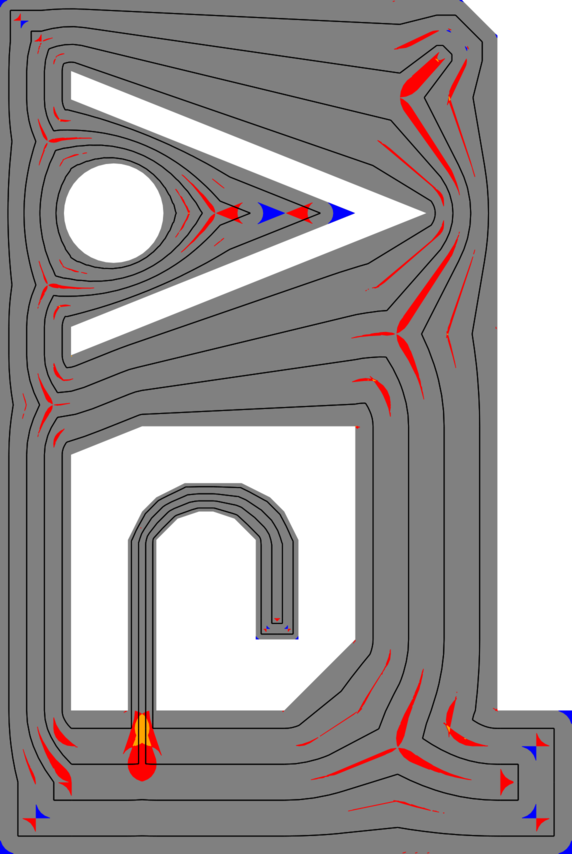
\includegraphics[height=\figheight]{sources/validation/gMAT_example/TEST_Constant_accuracy.png}
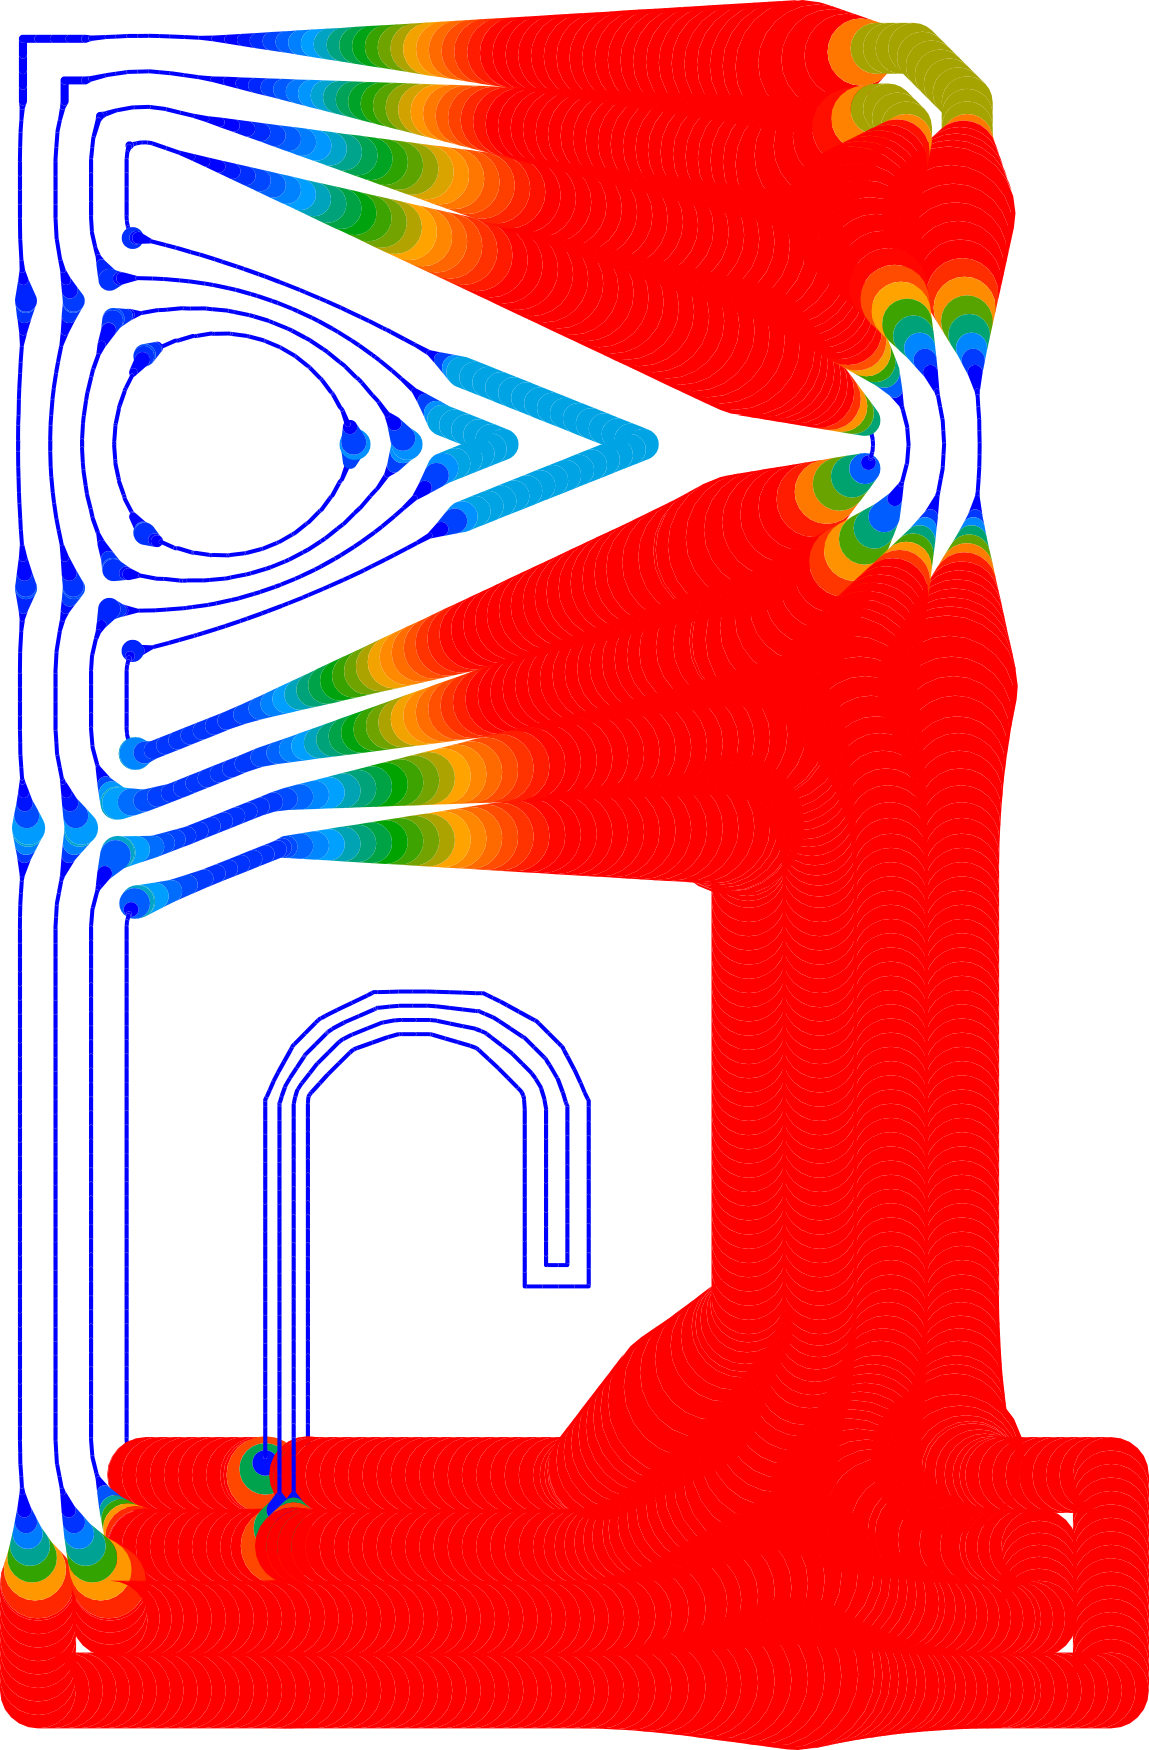
\includegraphics[height=\figheight]{sources/validation/gMAT_example/TEST_Constant_widths.png}
\caption{Constant}\label{TEST_Constant_accuracy}
\end{subfigure}
\begin{subfigure}{\figwidth}\centering
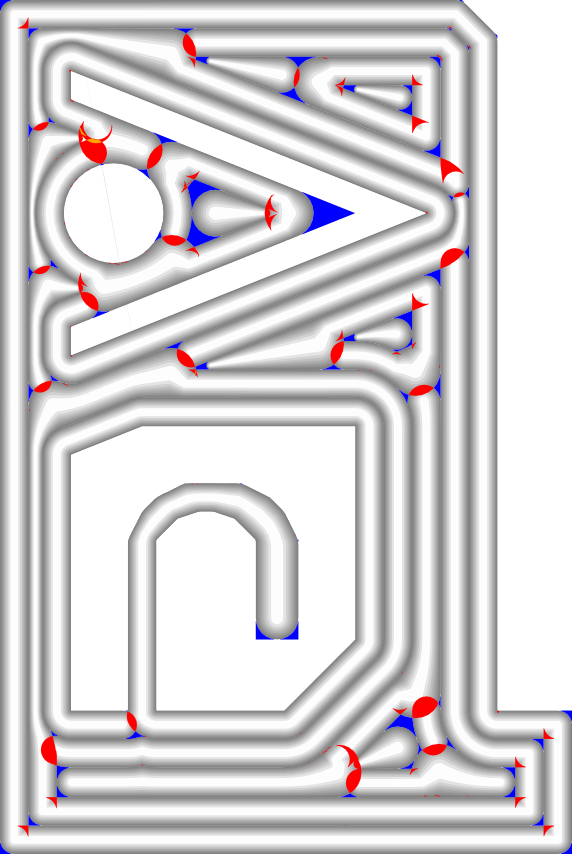
\includegraphics[height=\figheight]{sources/validation/gMAT_example/TEST_Center_accuracy.png}
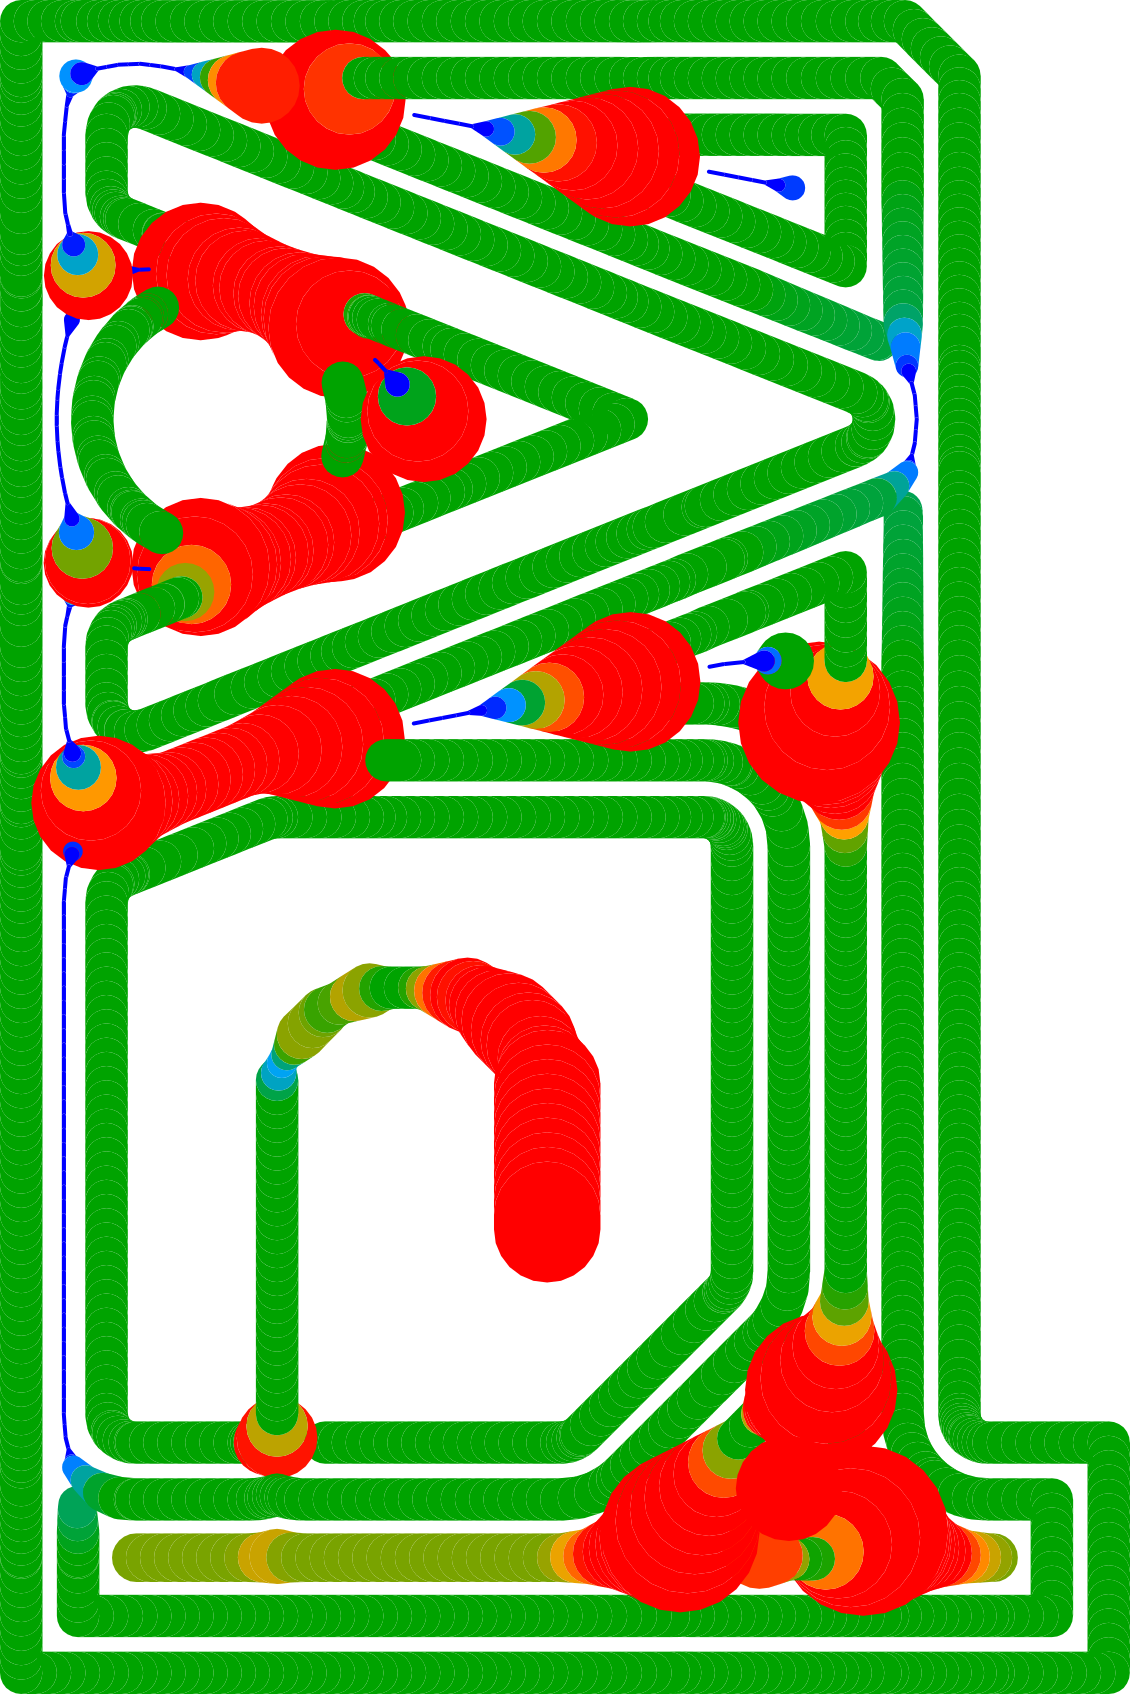
\includegraphics[height=\figheight]{sources/validation/gMAT_example/TEST_Center_widths.png}
\caption{Center}\label{TEST_Center_accuracy}
\end{subfigure}
\begin{subfigure}{\figwidth}\centering
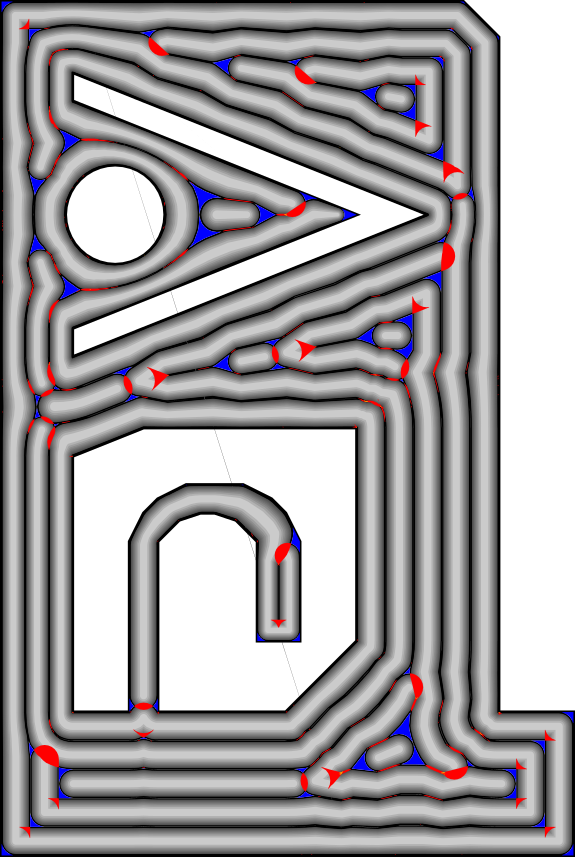
\includegraphics[height=\figheight]{sources/validation/gMAT_example/TEST_Distributed_accuracy.png}
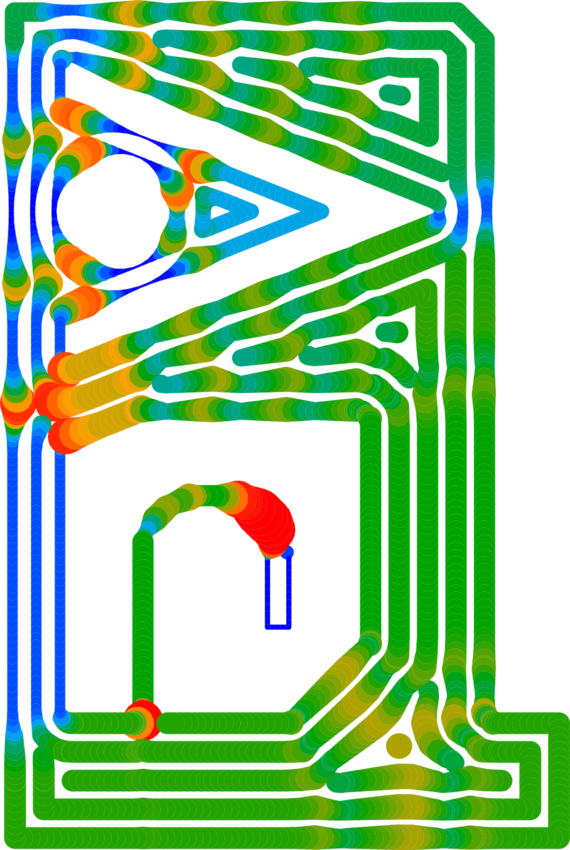
\includegraphics[height=\figheight]{sources/validation/gMAT_example/TEST_Distributed_widths.png}
\caption{Distributed}\label{TEST_Distributed_accuracy}
\end{subfigure}
\begin{subfigure}{\figwidth}\centering
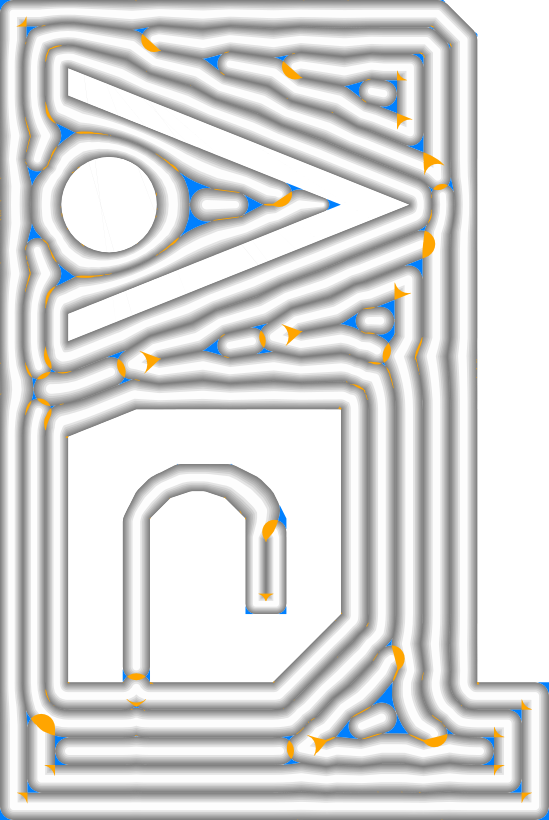
\includegraphics[width=\columnwidth]{sources/validation/gMAT_example/TEST_InwardDistributed_accuracy.png}
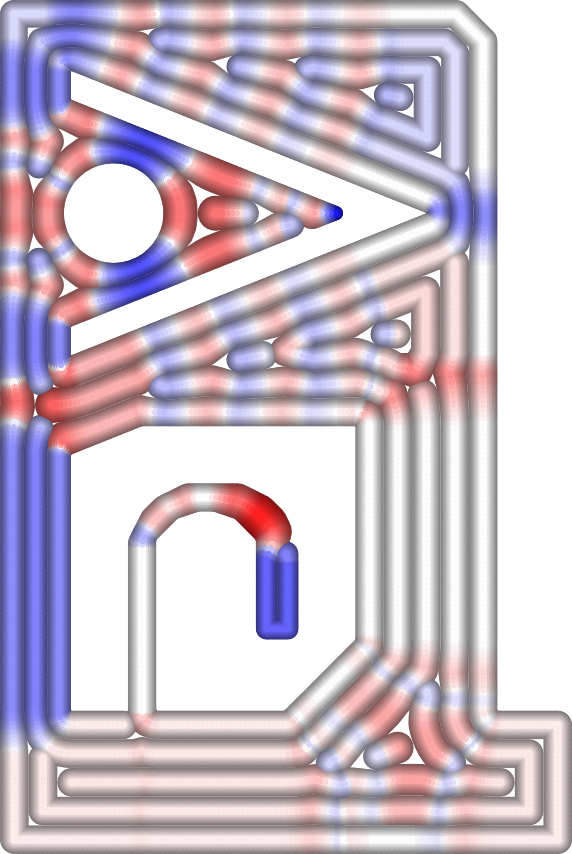
\includegraphics[width=\columnwidth]{sources/validation/gMAT_example/TEST_InwardDistributed_widths.png}
\caption{Inward}\label{TEST_InwardDistributed_accuracy}
\end{subfigure}
\begin{subfigure}{.04\columnwidth}\centering
\vspace{4cm}
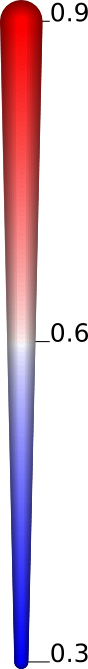
\includegraphics[height=\figheight]{sources/validation/gMAT_example/widths_legend.png}
\end{subfigure}
\caption{
Visualizing the overfills and underfills and the exaggerated widths for various beading strategies.
Grey areas are covered by extruded material,
blue areas in the top images signify underfill regions,
red areas overfill,
orange areas triply extruded areas (double overfill).
The bottom visualized the bead widths at each location by exaggerating their widths.
Cold colors are narrower than the nozzle size and warm colors are wider than the nozzle size.
}
\label{visualized_accuracy}
\end{figure*}


\subsection{Strategies}
We can emulate a variety of toolpath generation methods from related literature by applying various beading strategies to our framework.


\paragraph{Naive Strategy}
Because the naive strategy never employs single line polyline segments, we disable marking edges using the significance measure by choosing the limit angle.
\begin{align*}
\alpha_\text{max} &= \SI{180}{\degree} \\
b(d) &= 2 \left\lfloor \frac{d}{ 2w_\text{pref}} + \frac12 \right\rfloor \\
W(n,d)_i &= w_\text{pref} \text{ for all } i 
%\\
%L(n,d)_i &= w_\text{pref} \left(i + \frac12 \right) \text{ for all } i < \frac12 n
\end{align*}


\paragraph{Only outer bead}
Emulates \cite{Moesen2011}. We don't reduce line segments in 3-way intersections.

$d_\text{max}^\text{intersection} = \SI{0}{\percent}$

\begin{align*}
t(n) &= 0 \\
b(d) &=
\begin{cases}
1 & \text{ if } d < w_\text{pref} \\
2 & \text{ otherwise } \\
\end{cases}
 \\
W(n,d)_i &= 
\begin{cases}
d & \text{ if } n = 1 \\
w_\text{pref} & \text{ otherwise } \\
\end{cases}
%\\
%L(n,d)_i &= 
%\begin{cases}
%d / 2 & \text{ if } n = 1 \\
%w_\text{pref} / 2 & \text{ otherwise } \\
%\end{cases}
\end{align*}


\paragraph{Constant bead count}
Emulates \cite{Ding2016a}. We unmark all outer segments.

\begin{align*}
\alpha_\text{max} &= \SI{180}{\degree} \\
b(d) &= C \\
W(n,d)_i &= d / n \text{ for all } i 
%\\
%L(n,d)_i &= d / n \left(i + \frac12 \right) \text{ for all } i < \frac12 n
\end{align*}

\paragraph{Deviating toolpath at center}
Emulates \cite{Jin2017}

$r_\text{min} = 0.8 w_\text{pref}$ and $r_\text{max} = 1.25 w_\text{pref}$

\begin{align*}
t(n) &= \frac12 w_\text{pref} \\
b^-(d) &= 2 \left\lfloor \frac{d}{ 2w_\text{pref}} + \frac12 \right\rfloor \\
b(d) &= b^-(d) +
\begin{cases}
-1 & \text{ if } b^-(d) w_\text{pref} - d > w_\text{pref} - r_\text{max} \\
1  & \text{ if }  b^-(d) w_\text{pref} - d < w_\text{pref} - r_\text{min} \\
0 & \text{ otherwise}
\end{cases}
\\
W(n,d)_i &= 
\begin{cases}
d - (n-1) w_\text{pref} &\text{ if } i = \frac12 (n-1) \\
w_\text{pref} &\text{ otherwise }
\end{cases}
%\\
%L(n,d)_i &= 
%\begin{cases}
%d / 2 & \text{ if } i = \frac12 (n-1) \\
%w_\text{pref} \left(i + \frac12 \right) & \text{ otherwise }
%\end{cases}
\end{align*}





\paragraph{Distributed strategy}
Distribute the overfill or underfill which would happen using a naive strategy over all beads.
This maximizes robustness and minimizes narrow beads qhich are difficult to print.


\begin{align*}
b(d) &= \left\lfloor \frac{d}{ w_\text{pref}} + \frac12 \right\rfloor \\
W(n,d)_i &= d / n \text{ for all } i 
%\\
%L(n,d)_i &= d / n (i + \frac12) \text{ for all } i < \frac12 n
\end{align*}


\paragraph{General distributed strategy}
Distribute the overfill or underfill which would happen using a naive strategy $E$ over all beads unevenly depending on some weighing function $M(n.d)$, which defines the portion of overfill or underfill which would occur in the naive strategy to distribute to each junction.


\begin{align*}
b(d) &= \left\lfloor \frac{d}{ w_\text{pref}} + \frac12 \right\rfloor \\
E(n,d) &= d - n w_\text{pref} \\
W(n,d)_i &= w_\text{pref} + E(n,d) \frac{M(n,d)_i}{\sum_{j=0}^{n-1} M(n,d)_j} \text{ for all } i 
%\\
%L(n,d)_i &= d / n (i + \frac12) \text{ for all } i < \frac12 n
\end{align*}


\todo{TODO: check $n$ vs $n-1$ everywhere when comparing indices and the total size! Largest index should be $n-1$, not $n$!}

\paragraph{Inward distributed strategy}
For example, we can choose 
$$M(n,d)_i = \max(0, 1 - \frac{1}{N^2} (i - (n-1)/2)^2 )$$
To distribute the hypothetical over-/underfill over the innermost $2N$ beads, and distribute most of it to the inner beads.
That way we limit the impact of the distributed strategy and have the nominal bead width $w_\text{pref}$ in regions farther away from the middle.
This helps if print settings for bead widths other than the prefered width aren't calibrated as well as the settings for $w_\text{pref}$.
Toolpaths with deviating widths might result in less dimensional accuracy on the outline and uncalibrated mechanical properties throughout the volume, so limiting the number of beads width deviating bead width might be beneficial.
\todo{Emphasize this point more. Put it in the abstract and conclusion.}

Determining what the optimal distribution scheme would be is left as future work.



\paragraph{Widening}
Complementary to any of these strategies we can enforce a minimum feature size at no extra cost in our framework.
Regions where the model is narrower than the nozzle size can be printed with a bead width larger than the model thickness.
We can simply override
\begin{align*}
W'(n,d)_1 &=
\begin{cases}
\max \left( w_\text{nozzle}  ,  W(n,d)_1 \right) & \text{ if } n = 1 \\
W(n,d)_1 & \text{ otherwise}
\end{cases}
\end{align*}





\subsection{Computational analysis}
Experiments were performed on an Intel Core i7-7500U CPU @ \SI{2.70}{\giga\hertz} using a single core and \SI{16.3}{\giga\byte} memory.
The naive method was implemented using the state-of-the-art polygon offset library called Clipper. \cite{johnson2014clipper}

\paragraph{Accuracy}
In order to estimate the overfill and underfill we need to accurately calculate the area covered by a single extrusion path.
If we would simply use a isosceles trapezoidal area with base lengths equal to the widths of the two end points of the segment we would get strange artifacts at corners in the toolpath.
We therefore visualize include a semi-circle with a diameter equal to the starting width in the one end, and exclude it at the other end, because it will be included in the next extrusion segment.
For polyline extrusion paths which are not closed, we also include the semi-circle corresponding to the extrusion width of the end-position.
In order to print such extrusion paths accurately, we can modulate the amount of material flow per millimeter based on this visualization model.
See \cref{segment_visualization}.

\begin{figure}
\centering
\setlength{\figwidth}{.25\columnwidth}
\begin{subfigure}{\figwidth}\centering
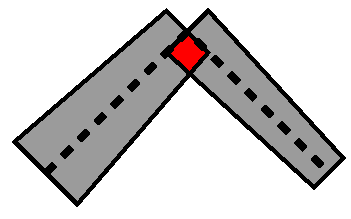
\includegraphics[width=\columnwidth]{sources/validation/visualization_principle_blocky.pdf}
\caption{Blocky}
\end{subfigure}
\begin{subfigure}{\figwidth}\centering
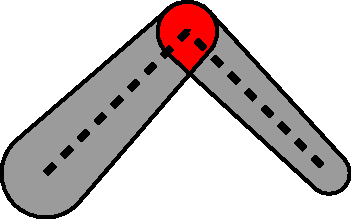
\includegraphics[width=\columnwidth]{sources/validation/visualization_principle_rounded.pdf}
\caption{Rounded}
\end{subfigure}
\begin{subfigure}{\figwidth}\centering
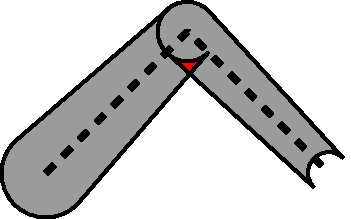
\includegraphics[width=\columnwidth]{sources/validation/visualization_principle_rounded_excluded.pdf}
\caption{Excluded}
\end{subfigure}
\caption{
Extruded area of two extrusion toolpath segments.
Red areas signify doubly extruded areas.
}
\label{segment_visualization}
\end{figure}

We can then estimate the amount of underfill by unioning the rounded visualization of all extrusion segments and then takign the difference from the original outline shape.
In order to deal with rounding errors we perform a morpholocial close of \SI{5}{\micro\meter} before calculating the total area of the underfill regions.

The overfill regions are calculated by adding the polygonal areas of each extrusion segment to a list.
We then add the original outline shape in reverse and perform a clipper operation which only keeps areas of positive winding order.
Because the reverse outline shape reduces the winding order of all extruded segments by one, we are left with the overfill areas.
In order to estimate the areas which are triply covered by extrusion segments, we repeat the process of adding the outline in reverse and performing the clipper operation.
These tripple extrusion areas count double toward the total amount of overfill.
The resulting overfill and underfill areas are visualzied for the different toolpath strategies in the top of \cref{visualized_accuracy}.


\todo{Zjenja should visualize overfill and underfill results in tables and/or graphs.}



\paragraph{Manufacturability}
Depending on the hardware configuration some bead widths are difficult to manufacture.
A bead width far below the nozzle size can result in fluttered extrusion, while a bead width far above the nozzle size can require pressures above the specifications of the machine.
\todo{Tim should put pictures of extremal bead widths in introduction!}
We visualize the bead widths resulting from the different strategies in an exaggerated manner in the bottom of \cref{visualized_accuracy}.





\subsection{Experimentation}
\todo{Tim will print objects and show qualities:}
\begin{itemize}
\item visual consistency of flat top skin surface
\item visual gradual transparency changes
\item graphs of tensile tests on thin walled object
\end{itemize}











